\section{Introduction}

\subsection{Motivations}

\begin{frame}[label=Motivations]
  \frametitle{Motivations}
  
  \textbf{Motivations :}
  \begin{itemize}
  \item étude du système \emph{Vélib'}
  \item problème : \emph{taux de foisonnement}
  
  (équilibre entre le nombre de places et le nombre de vélos disponibles)
  \end{itemize}
  
  \vfill
  \textbf{Cadre :}
  \begin{itemize}
  \item étude de complexité algorithmique
  \item N'est PAS une étude industrielle
  \end{itemize}

\end{frame}


\subsection{Modèle}

\begin{frame}[label=Modele]
  \frametitle{Modèle : Static Stations Balancing Problem (SSBP)}
  \framesubtitle{(Problème dérivée du \emph{C-delevery TSP})}
  
  \begin{center}
  
    \begin{minipage}[c]{.5\linewidth}
      \begin{center}
        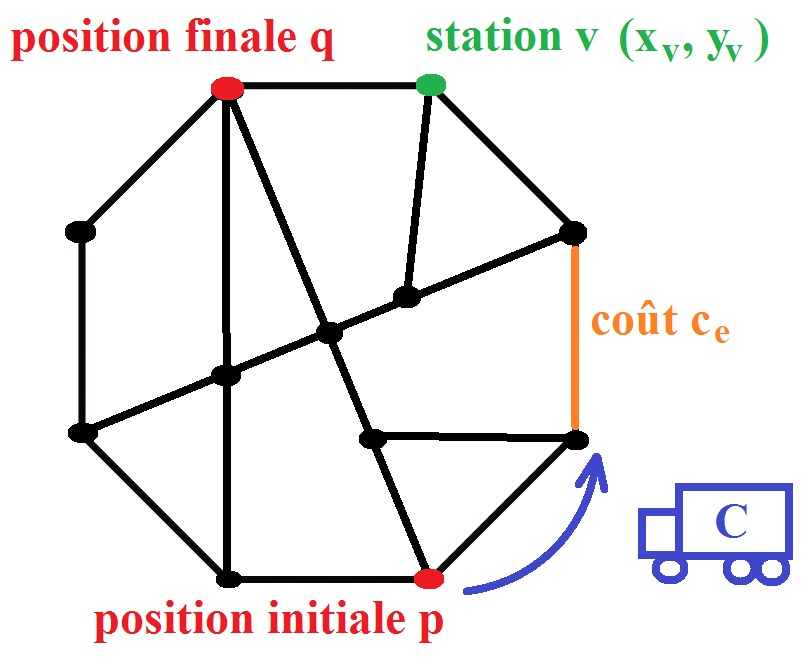
\includegraphics[width=\textwidth]{GrapheQuelconque.jpg}
      \end{center}
    \end{minipage}\hfill
    \begin{minipage}[c]{.5\linewidth}
      \textbf{Données.}
      \begin{itemize}
      \item graphe connexe $G=(V,E)$
      \item fonction de coût $\bs{c}$ sur les arêtes
      \item état initial $i$
        \begin{itemize}
        \item répartition initiale $\bs{x}$ des vélos
        \item position initiale du camion $p$
        \end{itemize}
      \item état cible $t$
        \begin{itemize}
        \item répartition cible $\bs{y}$ des vélos
        \item position finale du camion $q$
        \end{itemize}
      \item camion de capacité $C$
      \end{itemize}
    \end{minipage}
    
  \end{center}

  \pause
  
  \vfill
  \textbf{Tâche.} Trouver le coût minimal $\Upsilon_G$ de la séquence de mouvements permettant d'aller de l'état $i$ à l'état $t$ et le premier mouvement de cette séquence.

\end{frame}

\subsection{Résultats précédents}

\begin{frame}[label=PreviousResults]
  \frametitle{Résultats précédents}
  
  \begin{itemize}
  \item Graphe quelconque $\longrightarrow$ NP-difficile
  \item Graphe complet avec des coût unitaire $\longrightarrow$ NP-difficile
  \item \textcolor{red}{Arbre $\longrightarrow$ Linéaire en le nombre de sommets}
  \item Une borne inférieure du coût d'une solution optimale
  \end{itemize}

\end{frame}

\subsection{Cas étudié : le graphe circulaire}

\begin{frame}[label=GrapheCirculaire]
  \frametitle{Cas étudié : le graphe circulaire}
  
  \begin{center}
  
    \begin{minipage}[c]{.5\linewidth}
      \begin{center}
        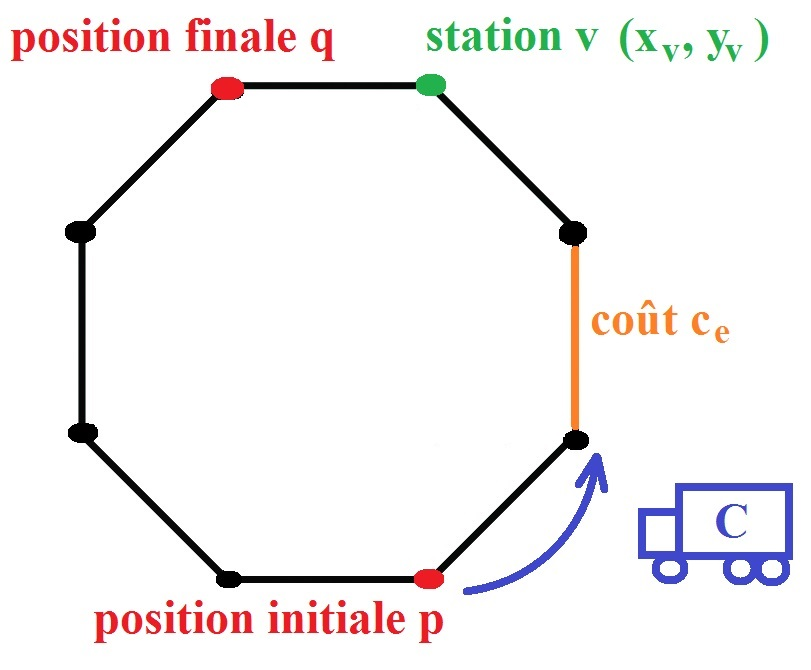
\includegraphics[width=\textwidth]{GrapheCirculaire.jpg}
        
        graphe \textcolor{red}{circulaire} $G=(V,E)$
      \end{center}
    \end{minipage}\hfill
    \begin{minipage}[c]{.5\linewidth}
      \textbf{Résultats obtenus :}
      \begin{itemize}
      \item Algorithme dans le cas triangulaire
      \item Algorithme polynomial dans le cas de la capacité infinie
      \item Conjecture dans un cas particulier de la capacité unitaire
      \end{itemize}
    \end{minipage}
    
  \end{center}

\end{frame}


